
\documentclass[letterpaper,hide notes,xcolor={table,svgnames},pdftex]{beamer}
\def\showexamples{t}


%\usepackage[svgnames]{xcolor}

%% Demo talk
%\documentclass[letterpaper,notes=show]{beamer}

\usecolortheme{crane}
\setbeamertemplate{navigation symbols}{}

\usetheme{MyPittsburgh}
%\usetheme{Frankfurt}

%\usepackage{tipa}

\usepackage{hyperref}
\usepackage{graphicx,xspace}
\usepackage[normalem]{ulem}

\newcommand\SF[1]{$\bigstar$\footnote{SF: #1}}



\newcounter{tmpnumSlide}
\newcounter{tmpnumNote}

% old question code
%\newcommand\question[1]{{$\bigstar$ \small \onlySlide{2}{#1}}}
% \newcommand\nquestion[1]{\ifdefined \presentationonly \textcircled{?} \fi \note{\par{\Large \textbf{?}} #1}}
% \newcommand\nanswer[1]{\note{\par{\Large \textbf{A}} #1}}


 \newcommand\mnote[1]{%
   \addtocounter{tmpnumSlide}{1}
   \ifdefined\showcues {~\tiny\fbox{\arabic{tmpnumSlide}}}\fi
   \note{\setlength{\parskip}{1ex}\addtocounter{tmpnumNote}{1}\textbf{\Large \arabic{tmpnumNote}:} {#1\par}}}

\newcommand\mmnote[1]{\note{\setlength{\parskip}{1ex}#1\par}}

%\newcommand\mnote[2][]{\ifdefined\handoutwithnotes {~\tiny\fbox{#1}}\fi
% \note{\setlength{\parskip}{1ex}\textbf{\Large #1:} #2\par}}

%\newcommand\mnote[2][]{{\tiny\fbox{#1}} \note{\setlength{\parskip}{1ex}\textbf{\Large #1:} #2\par}}

\newcommand\mquestion[2]{{~\color{red}\fbox{?}}\note{\setlength{\parskip}{1ex}\par{\Large \textbf{?}} #1} \note{\setlength{\parskip}{1ex}\par{\Large \textbf{A}} #2\par}\ifdefined \presentationonly \pause \fi}

\newcommand\blackboard[1]{%
\ifdefined   \showblackboard
  {#1}
  \else {\begin{center} \fbox{\colorbox{blue!30}{%
         \begin{minipage}{.95\linewidth}%
           \hspace{\stretch{1}} Some space intentionally left blank; done at the blackboard.%
         \end{minipage}}}\end{center}}%
         \fi%
}



%\newcommand\q{\tikz \node[thick,color=black,shape=circle]{?};}
%\newcommand\q{\ifdefined \presentationonly \textcircled{?} \fi}

\usepackage{listings}
\lstset{%
  keywordstyle=\bfseries,
  aboveskip=15pt,
  belowskip=15pt,
  captionpos=b,
  identifierstyle=\ttfamily,
  escapeinside={(*@}{@*)},
  stringstyle=\ttfamiliy,
  frame=lines,
  numbers=left, basicstyle=\scriptsize, numberstyle=\tiny, stepnumber=0, numbersep=2pt}

\usepackage{siunitx}
\newcommand\sius[1]{\num[group-separator = {,}]{#1}\si{\micro\second}}
\newcommand\sims[1]{\num[group-separator = {,}]{#1}\si{\milli\second}}
\newcommand\sins[1]{\num[group-separator = {,}]{#1}\si{\nano\second}}
\sisetup{group-separator = {,}, group-digits = true}

%% -------------------- tikz --------------------
\usepackage{tikz}
\usetikzlibrary{positioning}
\usetikzlibrary{arrows,backgrounds,automata,decorations.shapes,decorations.pathmorphing,decorations.markings,decorations.text}

\tikzstyle{place}=[circle,draw=blue!50,fill=blue!20,thick, inner sep=0pt,minimum size=6mm]
\tikzstyle{transition}=[rectangle,draw=black!50,fill=black!20,thick, inner sep=0pt,minimum size=4mm]

\tikzstyle{block}=[rectangle,draw=black, thick, inner sep=5pt]
\tikzstyle{bullet}=[circle,draw=black, fill=black, thin, inner sep=2pt]

\tikzstyle{pre}=[<-,shorten <=1pt,>=stealth',semithick]
\tikzstyle{post}=[->,shorten >=1pt,>=stealth',semithick]
\tikzstyle{bi}=[<->,shorten >=1pt,shorten <=1pt, >=stealth',semithick]

\tikzstyle{mut}=[-,>=stealth',semithick]

\tikzstyle{treereset}=[dashed,->, shorten >=1pt,>=stealth',thin]

\usepackage{ifmtarg}
\usepackage{xifthen}
\makeatletter
% new counter to now which frame it is within the sequence
\newcounter{multiframecounter}
% initialize buffer for previously used frame title
\gdef\lastframetitle{\textit{undefined}}
% new environment for a multi-frame
\newenvironment{multiframe}[1][]{%
\ifthenelse{\isempty{#1}}{%
% if no frame title was set via optional parameter,
% only increase sequence counter by 1
\addtocounter{multiframecounter}{1}%
}{%
% new frame title has been provided, thus
% reset sequence counter to 1 and buffer frame title for later use
\setcounter{multiframecounter}{1}%
\gdef\lastframetitle{#1}%
}%
% start conventional frame environment and
% automatically set frame title followed by sequence counter
\begin{frame}%
\frametitle{\lastframetitle~{\normalfont(\arabic{multiframecounter})}}%
}{%
\end{frame}%
}
\makeatother

\makeatletter
\newdimen\tu@tmpa%
\newdimen\ydiffl%
\newdimen\xdiffl%
\newcommand\ydiff[2]{%
    \coordinate (tmpnamea) at (#1);%
    \coordinate (tmpnameb) at (#2);%
    \pgfextracty{\tu@tmpa}{\pgfpointanchor{tmpnamea}{center}}%
    \pgfextracty{\ydiffl}{\pgfpointanchor{tmpnameb}{center}}%
    \advance\ydiffl by -\tu@tmpa%
}
\newcommand\xdiff[2]{%
    \coordinate (tmpnamea) at (#1);%
    \coordinate (tmpnameb) at (#2);%
    \pgfextractx{\tu@tmpa}{\pgfpointanchor{tmpnamea}{center}}%
    \pgfextractx{\xdiffl}{\pgfpointanchor{tmpnameb}{center}}%
    \advance\xdiffl by -\tu@tmpa%
}
\makeatother
\newcommand{\copyrightbox}[3][r]{%
\begin{tikzpicture}%
\node[inner sep=0pt,minimum size=2em](ciimage){#2};
\usefont{OT1}{phv}{n}{n}\fontsize{4}{4}\selectfont
\ydiff{ciimage.south}{ciimage.north}
\xdiff{ciimage.west}{ciimage.east}
\ifthenelse{\equal{#1}{r}}{%
\node[inner sep=0pt,right=1ex of ciimage.south east,anchor=north west,rotate=90]%
{\raggedleft\color{black!50}\parbox{\the\ydiffl}{\raggedright{}#3}};%
}{%
\ifthenelse{\equal{#1}{l}}{%
\node[inner sep=0pt,right=1ex of ciimage.south west,anchor=south west,rotate=90]%
{\raggedleft\color{black!50}\parbox{\the\ydiffl}{\raggedright{}#3}};%
}{%
\node[inner sep=0pt,below=1ex of ciimage.south west,anchor=north west]%
{\raggedleft\color{black!50}\parbox{\the\xdiffl}{\raggedright{}#3}};%
}
}
\end{tikzpicture}
}


%% --------------------

%\usepackage[excludeor]{everyhook}
%\PushPreHook{par}{\setbox0=\lastbox\llap{MUH}}\box0}

%\vspace*{\stretch{1}

%\setbox0=\lastbox \llap{\textbullet\enskip}\box0}

\setlength{\parskip}{\fill}

\newcommand\noskips{\setlength{\parskip}{1ex}}
\newcommand\doskips{\setlength{\parskip}{\fill}}

\newcommand\xx{\par\vspace*{\stretch{1}}\par}
\newcommand\xxs{\par\vspace*{2ex}\par}
\newcommand\tuple[1]{\langle #1 \rangle}
\newcommand\code[1]{{\sf \footnotesize #1}}
\newcommand\ex[1]{\uline{Example:} \ifdefined \presentationonly \pause \fi
  \ifdefined\showexamples#1\xspace\else{\uline{\hspace*{2cm}}}\fi}

\newcommand\ceil[1]{\lceil #1 \rceil}


\AtBeginSection[]
{
   \begin{frame}
       \frametitle{Outline}
       \tableofcontents[currentsection]
   \end{frame}
}



\pgfdeclarelayer{edgelayer}
\pgfdeclarelayer{nodelayer}
\pgfsetlayers{edgelayer,nodelayer,main}

\tikzstyle{none}=[inner sep=0pt]
\tikzstyle{rn}=[circle,fill=Red,draw=Black,line width=0.8 pt]
\tikzstyle{gn}=[circle,fill=Lime,draw=Black,line width=0.8 pt]
\tikzstyle{yn}=[circle,fill=Yellow,draw=Black,line width=0.8 pt]
\tikzstyle{empty}=[circle,fill=White,draw=Black]
\tikzstyle{bw} = [rectangle, draw, fill=blue!20, 
    text width=4em, text centered, rounded corners, minimum height=2em]
    
    \newcommand{\CcNote}[1]{% longname
	This work is licensed under the \textit{Creative Commons #1 3.0 License}.%
}
\newcommand{\CcImageBy}[1]{%
	\includegraphics[scale=#1]{creative_commons/cc_by_30.pdf}%
}
\newcommand{\CcImageSa}[1]{%
	\includegraphics[scale=#1]{creative_commons/cc_sa_30.pdf}%
}
\newcommand{\CcImageNc}[1]{%
	\includegraphics[scale=#1]{creative_commons/cc_nc_30.pdf}%
}
\newcommand{\CcGroupBySa}[2]{% zoom, gap
	\CcImageBy{#1}\hspace*{#2}\CcImageNc{#1}\hspace*{#2}\CcImageSa{#1}%
}
\newcommand{\CcLongnameByNcSa}{Attribution-NonCommercial-ShareAlike}

\newenvironment{changemargin}[1]{% 
  \begin{list}{}{% 
    \setlength{\topsep}{0pt}% 
    \setlength{\leftmargin}{#1}% 
    \setlength{\rightmargin}{1em}
    \setlength{\listparindent}{\parindent}% 
    \setlength{\itemindent}{\parindent}% 
    \setlength{\parsep}{\parskip}% 
  }% 
  \item[]}{\end{list}} 




\title{Lecture 9 --- Version Control}

\author{Jeff Zarnett \& Patrick Lam \\ \small \texttt{jzarnett@uwaterloo.ca \& p.lam@ece.uwaterloo.ca}}
\institute{Department of Electrical and Computer Engineering \\
  University of Waterloo}
\date{\today}

\begin{document}

\begin{frame}
  \titlepage

\end{frame}

\begin{frame}
\frametitle{Version Control}

\begin{changemargin}{1cm}
\Large
Ever wanted to undo your changes to software? \\[1em]
Ever needed to collaborate with others to develop software?
\begin{center}

\includegraphics[width=.4\textwidth]{images/no-outlook}\mnote{without
having to email new versions of files to each other and manually integrate
changes?}
\end{center}
\end{changemargin}

\end{frame}

\begin{frame}
\frametitle{Conceptual Idea}

\begin{center}
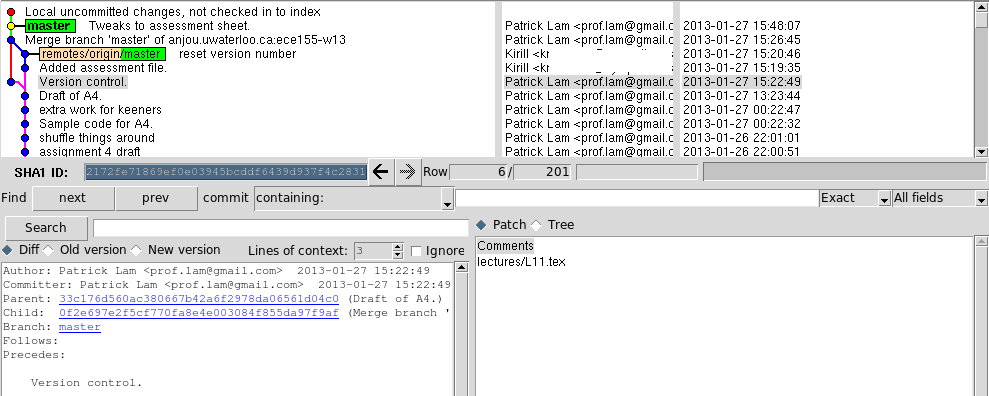
\includegraphics[width=.7\textwidth]{images/git}
\end{center}

\begin{changemargin}{1cm}
\begin{itemize}
\item Store a \structure{repository} of \structure{revisions}.\\[1em]
Each revision is a snapshot of a set of files.
\item Can search by author, date, commit comment.
\item Can revert to previous revisions.
\end{itemize}
\end{changemargin}
\end{frame}


\begin{frame}
\frametitle{Without Version Control}
\begin{changemargin}{1cm}

\begin{center}
	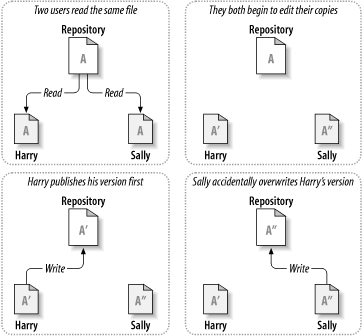
\includegraphics[width=.65\textwidth]{images/ch02dia2.png}
	\hfill {\tiny \url{http://svnbook.red-bean.com/en/1.6/svn.basic.version-control-basics.html}} 
\end{center}

\mnote{Bugs that were fixed would come back again, new features would break, and so on. There could be a central person whose sole job it is to integrate changes from each developer, but this doesn't scale very well and wastes a lot of human effort. Solution: version control.}

\end{changemargin}
\end{frame}

\begin{frame}
\frametitle{Lock-Modify-Unlock}

\begin{changemargin}{1cm}
The first model: \alert{Lock-Modify-Unlock} \mnote{To edit a file, you need to lock it - you get exclusive access to change the file. Next, you modify the files. You can only modify files you have locked. Finally, when you are done, you unlock the file and it's available for others to lock.}


Considered obsolete, but worth learning about.

\end{changemargin}
\end{frame}

\begin{frame}
\frametitle{Lock-Modify-Unlock}
\begin{changemargin}{1cm}

\begin{center}
	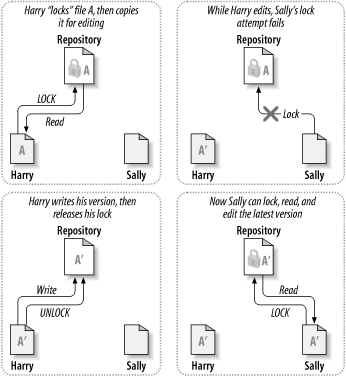
\includegraphics[width=.65\textwidth]{images/ch02dia3.png}
	\hfill {\tiny \url{http://svnbook.red-bean.com/en/1.6/svn.basic.version-control-basics.html}} 
\end{center}

\mnote{Note that when a file is locked, nobody else can lock it until you unlock it (see step 3), ensuring that there is only one person who has write access to the file at a time (i.e., no concurrent modification)}

\end{changemargin}
\end{frame}

\begin{frame}
\frametitle{Problems with Lock-Modify-Unlock}
\begin{changemargin}{1cm}

\begin{itemize}
	\item Forgot to Unlock. \mnote{ Locking also requires timely unlocking - if Harry has locked a file, and forgotten to unlock it before he left for vacation, Sally is stuck - she will have to get an administrator to unlock the file for her.}
	\item Unnecessary Waiting \mnote{Suppose the two developers need to edit the same file but their changes do not overlap. It would be nice if Harry can change the beginning of the file and Sally can change the end, without having to wait for one to finish before the next one starts. With lock-modify-unlock, Sally simply has to wait to make her changes until she can lock the file.}
	\item Deadlock \mnote{Suppose Harry has \texttt{file1} locked and discovers he needs to also lock \texttt{file2}. He cannot, however, because Sally has \texttt{file2} locked and she wants to get \texttt{file1}. This situation is known as a \emph{deadlock} when it happens in a computer system - and there must be a process for resolving this.}
	\item Parallel Modification \mnote{if Harry is editing \texttt{file1} and Sally is editing \texttt{file2}. Their changes don't overlap directly, but if the two files interact it's possible that they've made the two files incompatible with one another.}
\end{itemize}

\end{changemargin}
\end{frame}

\begin{frame}
\frametitle{Copy-Modify-Merge}

\begin{changemargin}{1cm}
The current model: \alert{Copy-Modify-Merge} \mnote{To start working on a project, you check out (\emph{copy}) a
  version of the project, usually the most recent one, to create your
  working copy.
Next, you \emph{modify} your copy of the projects, test your
  changes, and commit your changes to the repository.
Other developers can then \emph{merge} your changes into their
  working copies, which contain their changes. They will then commit
  their changes as appropriate.}


Yes, merging works. Have you tried it?

\end{changemargin}
\end{frame}

\begin{frame}
\frametitle{Copy-Modify-Merge}
\begin{changemargin}{1cm}

\begin{center}
	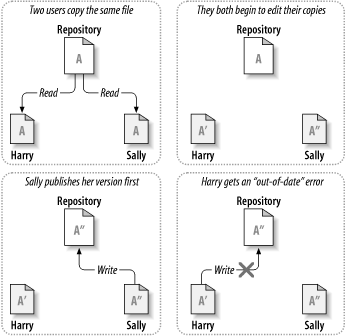
\includegraphics[width=.65\textwidth]{images/ch02dia4.png}
	\hfill {\tiny \url{http://svnbook.red-bean.com/en/1.6/svn.basic.version-control-basics.html}} 
\end{center}

\mnote{In this situation, Harry and Sally each got a copy of file \texttt{A}. Sally finished her changes first and committed those changes, which updates the repository version of \texttt{A}. Then Harry finishes. But he cannot submit his changes to the repository because the version of \texttt{A} has changed in the meantime. So he needs to perform a merge.}

\end{changemargin}
\end{frame}

\begin{frame}
\frametitle{Copy-Modify-Merge}
\begin{changemargin}{1cm}
\begin{center}
	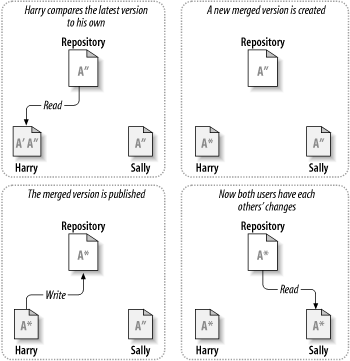
\includegraphics[width=.65\textwidth]{images/ch02dia5.png}
	\hfill {\tiny \url{http://svnbook.red-bean.com/en/1.6/svn.basic.version-control-basics.html}} 
\end{center}

\mnote{Changes from the repository version of \texttt{A} are downloaded and the changes Sally made need to be combined with Harry's changes to produce the newest version of \texttt{A}, shown as \texttt{A''}.}

\end{changemargin}
\end{frame}

\begin{frame}
\frametitle{Merging}
\begin{changemargin}{1cm}
Usually succeeds automatically.

Sometimes you will have to solve a conflict manually.

Consider: the common ancestor, your change, and the other change.

Advantage of C-M-M: More parallelism. Conflicts infrequent.

\end{changemargin}
\end{frame}

\begin{frame}
\frametitle{CVS}
\begin{changemargin}{1cm}
One of the first version control systems: \alert{cvs}\mnote{Concurrent Versioning System}

Developed in the 1980s; mature technology

Introduced the concept of \alert{branches}. \mnote{Revision control sometimes uses the terminology of trees to describe the relationships between different revisions. The main line of the code is called the \emph{trunk}, \emph{main}, or \emph{master}. A parallel line is called a \emph{branch}.}

Branches split off from the \alert{trunk} (mainline). \mnote{Branches are sometimes merged into their parent (the mainline, usually) which incorporates all of those changes back into the mainline. However, branches may be long-running, such as when Ubuntu creates a release (like 13.04). In this case, changes like bug fixes may be submitted to both the trunk and the branch. This kind of branch will not get merged with the trunk.}


\end{changemargin}
\end{frame}

\begin{frame}
\frametitle{CVS: Shortcomings}
\begin{changemargin}{1cm}

\begin{itemize}
	\item No Moving/Renaming Support \mnote{A file that is moved or renamed in \texttt{cvs} is treated as if the old file was deleted and a new file created, so all history information is lost.}
	\item Branches Expensive \mnote{Creating a new branch is expensive and not well supported if the branch is expected to go on for a long time (such as being a supported software release).}
	\item Commits Not Atomic \mnote{If something goes wrong during a commit, it's possible the repository will be in a corrupted state (with some files changed and others unchanged). If commits are \texttt{atomic}, either the whole commit succeeds or it's cancelled and rolled back to the state before the commit was applied.}
\end{itemize}


\end{changemargin}
\end{frame}

\begin{frame}
\frametitle{From CVS to SVN}
\begin{changemargin}{1cm}

Attempts to address these problems led to: Subversion (\alert{svn}).


\end{changemargin}
\end{frame}

\begin{frame}

\frametitle{Case Study: Subversion}

\begin{center}
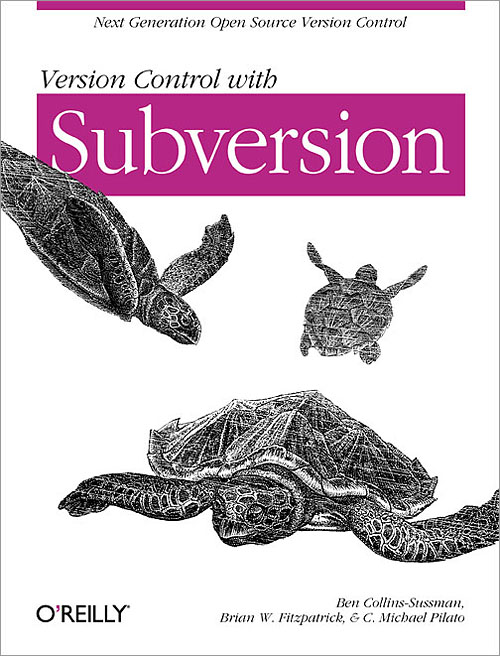
\includegraphics[height=0.7\textheight]{images/subversion}
\end{center}
\hfill \url{(http://svnbook.red-bean.com/)}

You are using Subclipse; I'll talk about command-line usage.
\end{frame}

\begin{frame}[fragile]

\frametitle{Creating a new repository}

\begin{changemargin}{2.5cm}
Create one from scratch:

{\scriptsize \begin{verbatim}  svnadmin create c:\svn\repos\end{verbatim}}

~\\[1em]
More commonly, check out a repository:
\end{changemargin}

{\scriptsize \begin{verbatim}  svn checkout http://k9mail.googlecode.com/svn/k9mail/trunk/
      k9mail-read-only\end{verbatim}}

\begin{changemargin}{2.5cm}
\begin{itemize}
\item creates a \structure{working copy}. (You've done this.)
\end{itemize}
\end{changemargin}

\end{frame}
\begin{frame}
\frametitle{Adding and Ignoring Files}
\begin{changemargin}{1cm}
You've seen how to add files to the repository \\~~~(Team \textgreater~Add to Version Control).\\

command-line: {\tt svn add filename}\\

\begin{itemize}
\item failure to add files: leading cause of build breakage
\end{itemize}

You've seen ignored files like {\tt R.java}.

\begin{itemize}
\item Generally, do \alert{not} commit generated files!
\end{itemize}
Instead, tell Subversion to ignore them, \\ ~~~~e.g. using wildcards.

\end{changemargin}
\end{frame}

\begin{frame}
\frametitle{Committing Files}
\begin{changemargin}{1cm}
\large

On SVN, a commit makes your changes available to the world.\\
In decentralized version control, a commit records current version.\\[1em]

\structure{When to commit?}

\begin{itemize}
\item \alert{What you commit must compile!}
\item Generally, one feature at a time, after testing. (Varies by source control system.)
\end{itemize}

\end{changemargin}
\end{frame}

\begin{frame}[fragile]
\frametitle{Commit Messages}

\begin{changemargin}{1cm}
\begin{itemize}
\item An important form of project documentation\footnote{\tiny \url{http://who-t.blogspot.ca/2009/12/on-commit-messages.html}, accessed 27Jan13}.
\end{itemize}
~\\[1em]

Start with a one-line summary.\\[1em]

Establish the specific context of the change:
\begin{itemize}
\item Why is it necessary?
\item How does it work?
\item What are the effects?
\end{itemize}

Meta-commit message\footnote{\tiny \url{https://github.com/erlang/otp/wiki/Writing-good-commit-messages}, accessed 27Jan13}:
\end{changemargin}

{\small
\begin{verbatim}
Summarize clearly in one line what the commit is about

Describe the problem the commit solves or the use
case for a new feature. Justify why you chose
the particular solution.
\end{verbatim}
}

\end{frame}

\begin{frame}[fragile]
\frametitle{Updating your repository}

\Large
\begin{changemargin}{1cm}
Pull changes from
the repository to your working copy. \\[1em]

Use {\tt svn update} to do that.
If all goes well, you'll get output like this:\\[1em]

{\scriptsize
\begin{verbatim}
plam@noether:~/production/11.aosd.modularity$ svn up
D    example.tex
A    studies.tex
U    introduction.tex
A    sketch.tex
U    main.tex
\end{verbatim}
}
\end{changemargin}

\end{frame}

\begin{frame}[fragile]
\frametitle{Conflicts: the bane of your existence}

\begin{changemargin}{1cm}
This is a pain:
{\scriptsize
\begin{verbatim}
plam@noether:~/production/11.aosd.modularity$ svn up
C    example.tex
\end{verbatim}
}
~\\[1em]

Why? 
\begin{itemize}
\item Both the latest version and your version differ
from the common ancestor.
\end{itemize}
\end{changemargin}
\end{frame}

\begin{frame}[fragile]
\frametitle{Example conflict}

\begin{changemargin}{1cm}
How?
\begin{enumerate}
\item I wrote: ``Here's a line of text''. 
\item Programmer X changes it to ``Here's a line of text that I modified.''
\item I change it again to ``Here's a modified line of text.''
\end{enumerate}
~\\[1em]

The result:
\begin{verbatim}
<<<<<<< HEAD
Here's a line of text that I modified.
=======
Here's a modified line of text.
>>>>>>> zzz
\end{verbatim}

~\\
You need to fix it and tell SVN that you've fixed it.

\end{changemargin}

\end{frame}

\begin{frame}
\frametitle{Stepping Back in Time}

\Large
\begin{changemargin}{1cm}
Major win of version control:
\begin{itemize}
\item can undo sketchy changes.
\end{itemize}
~\\
Can update to a past revision number or a~date/time.\\[1em]

How to know which version to revert to?\\
\begin{itemize}
\item your detailed log messages!
\end{itemize}
~\\

Note: you can't commit an update, but you can merge it to your working
copy.
\end{changemargin}
\end{frame}

\begin{frame}[fragile]
\frametitle{Diffs}

\Large
\begin{changemargin}{1cm}
Basic unit of version control is the diff:

\begin{itemize}
\item describes what's \structure{different} between two versions.
\end{itemize}

Inspect your diffs before committing. Commit minimal diffs.

{\tiny 
\hspace*{4em} 
\begin{verbatim}
===================================================================
--- Text/abstract.tex	(revision 17379)
+++ Text/abstract.tex	(working copy)
@@ -1,10 +1,10 @@
 Runtime monitoring enables developers to (1) specify important program
 properties and (2) dynamically validate that these properties hold.
 In recent research, we have found that static analysis techniques can,
-in many cases, verify that runtime monitors never trigger.  In
-this paper, we describe a system which enables developers to visualize
-the remaining cases---potential
+in many cases, verify that runtime monitors never trigger.  In this
+paper, we describe a tool which enables developers to visualize the
+remaining cases---potential points
\end{verbatim}
}
\end{changemargin}
\end{frame}


\begin{frame}
\frametitle{Basic SVN Workflow}

\begin{changemargin}{1cm}
Repeat until done:
\begin{itemize}
\item Update your working copy.\\ ~~({\tt svn update})
\item Edit files. Manipulate tracked files.\\ ~~({\tt svn add, svn rm, svn copy, svn move})
\item Examine changes.\\~~({\tt svn status, svn diff})
\item Undo changes, if necessary.\\~~({\tt svn revert})
\item Commit changes to the server.\\~~({\tt svn commit})
\end{itemize}
\end{changemargin}

\end{frame}

\begin{frame}
\frametitle{SVN vs CVS}
\begin{changemargin}{1cm}
SVN was specifically intended to address the shortcomings of CVS. Some properties:
\begin{itemize}
	\item Atomic Commits \mnote{If something goes wrong during a commit, it's possible the repository will not be in a corrupted state. Either the entire commit succeeds or the whole thing is rolled back.}
	\item Branch Operations \mnote{Branch operations are much less expensive, and there is no longer an expectation that a branch gets merged into the trunk sooner rather than later.}
	\item Support for Moving or Renaming \mnote{A file that is moved or renamed in svn is handled better than it was in cvs, but it's still got some issues.}
\end{itemize}
\end{changemargin}
\end{frame}

\begin{frame}
\frametitle{SVN vs CVS}
\begin{changemargin}{1cm}
SVN was specifically intended to address the shortcomings of CVS. Some properties:
\begin{itemize}
	\item Atomic Commits \mnote{If something goes wrong during a commit, it's possible the repository will not be in a corrupted state. Either the entire commit succeeds or the whole thing is rolled back.}
	\item Branch Operations \mnote{Branch operations are much less expensive, and there is no longer an expectation that a branch gets merged into the trunk sooner rather than later.}
	\item Support for Moving or Renaming \mnote{A file that is moved or renamed in svn is handled better than it was in cvs, but it's still got some issues.}
\end{itemize}
\end{changemargin}
\end{frame}

\begin{frame}
\frametitle{Issues with SVN}
\begin{changemargin}{1cm}
Subversion is better than CVS, but it still has some problems:
\begin{itemize}
	\item Centralized \mnote{In svn, users all connect to the central repository. If network access is unavailable, none of the source control operations can take place (update, look in the logs, commit, et cetera). }
	\item Slow \mnote{It's unfortunately common that both cvs and svn take long enough to do an update of a large amount of source code that it leaves plenty of time for a developer to go get a cup of coffee...}

\end{itemize}
\end{changemargin}
\end{frame}

\begin{frame}
\frametitle{Centralized vs. Distributed}
\begin{changemargin}{1cm}
Traditionally, there was one canonical central repository for a software project.

\alert{Centralized systems} work on that model.

Newer version control systems can be \alert{decentralized}. \mnote{Every
developer can keep a full copy of the project's history on their
system, and there doesn't need to be a central repository anymore
(although one often exists, in some sense). You can therefore commit
changes to the history on your local computer, without network access.}

\end{changemargin}
\end{frame}

\begin{frame}
\frametitle{Git and Mercurial}
\begin{changemargin}{1cm}
One of those decentralized systems is \texttt{git}.

Designed to be a new model, not just ``better'' \texttt{svn}.

Created by Linus Torvalds (yes, of the Linux Kernel).

\end{changemargin}
\end{frame}

\begin{frame}
\frametitle{Git}
\begin{changemargin}{1cm}
Decentralized -- can view everything offline.

Fast! \mnote{Operations are often dramatically faster (because they are done on the local disk and not over the network)}

Branch operations inexpensive and recommended workflow.

Similar to svn: add, ignore, commit, update, merge, resolve, etc.

Complex (steep learning curve)
\end{changemargin}
\end{frame}


\begin{frame}
\frametitle{Git Workflow}
\begin{changemargin}{1cm}
The basic work cycle of git is the following:
\begin{itemize}
\item Update working copy of the repository ({\tt git pull}).
\item Create a feature branch ({\tt git checkout -b}).
\item Edit files. Manipulate set of files with {\tt git add}, {\tt git rm}.
\end{itemize}

\end{changemargin}
\end{frame}

\begin{frame}
\frametitle{Git Workflow}
\begin{changemargin}{1cm}
\begin{itemize}
\item Examine changes ({\tt git status}, {\tt git diff}).
\item Undo changes ({\tt git checkout}, {\tt git reset}).
\item Commit changes ({\tt git commit}).
\item Merge your feature branch into the parent branch:
 \begin{itemize}
 \item Check the parent branch out ({\tt git checkout})
 \item {\tt git pull} to update
 \item merge ({\tt git merge}).
 \end{itemize}
\item Finally, share your changes with others using {\tt git push}.
\end{itemize}

\end{changemargin}
\end{frame}

\begin{frame}
\frametitle{Mercurial}
\begin{changemargin}{1cm}
About Mercurial (\texttt{hg})

Distributed like \texttt{git}.

Easier to learn; similar to \texttt{svn}.

Better Windows support.

Can be used alongside git on the same repository.

\end{changemargin}
\end{frame}

\end{document}
